%----------------------------------------------------------------------------
\chapter{Optical Character Recognition}

This chapter focuses on the OCR (Optical Character Recognition) part of the ALPR process. I propose a lightweight algorithm that is part of a vehicle identification pipeline capable of running on Android smartphones.

\section{Related Work}

There are two main approaches regarding Optical Character Recognition with deep learning. Object detection can be used to locate individual characters on images. This solution outputs a character score for each detected box, instantly recognizing tokens in multiline plates. However, there are significant drawbacks in the context of OCR\cite{CTCexp}:

\begin{itemize}
  \item Annotating real-life datasets on a character level can be time-consuming.
  \item Detectors usually struggle with small objects (like characters in text).
  \item The outputs are character scores, and therefore further pre-processing is needed to get the final text from it.
  \item When using fixed boxes, a single character can trigger multiple positions. What if ``GGOO'' is the prediction because the ``O'' is a wide-character? We must remove all duplicate tokens. Nevertheless, it can be that the original text would have been ``GGO''. Then removing the duplicates produces a wrong result.
\end{itemize}

Another approach can be the sequential feature extraction with convolutional and recurrent layers guided by Connectionist Temporal Classification\cite{CTC}. In this solution, the convolutional part extracts the necessary features. Then the recurrent part processes them sequentially to output a probability for each time step. The main advantage over the object detection approach is that only an image and the target text need to be provided; CTC handles the rest. Therefore, character positions and width are ignored, which makes it easier to label real-life datasets. An output sequence of a CRNN can be easily translated into a text with either the Greedy or Beam search algorithms, as CTC also indicates the end of the characters with a specific token. However, these solutions can process images along one axis (practically horizontally); therefore, they cannot recognize multiline blocks in standalone versions.

Different approaches exist to convert CRNNs into multiline recognizers. The classical solution can be the Scale Space Technique for Word Segmentation\cite{ScaleWordSeg}, which outputs block positions. It performs relatively well (87\%) on handwritten papers. For multiple text block recognition, both an object detector or an image segmentation model can be used first, and their outputs then fed into the CRNN. However, this solution is wasteful as an image must be processed multiple times, and low-level feature extractions are not shared across individual networks. Recently, Wojna et al.\cite{Attention-basedExtract} proposed an end-to-end model with an attention mechanism. OrigamiNet\cite{OrigamiNet} introduced a one-step model by learning to unfold, transforming existing CRNNs into multiline recognizers. Other approaches still exist, like proposed by WPOD-NET\cite{WPOD-NET}, where a modified YOLO detector is used for OCR purposes.

\section{Data}

An adequate amount of data is required to train a deep learning algorithm. There is no generally available de-facto benchmark dataset in ALPR. There were plate sets mainly for object detection (which were missing text labels). The OCR sets neither satisfied the search as they were too specific in domains like handwriting recognition or housing numbers. A good option where there are 15 million annotated images is the database of platesmania.com\cite{PlatesMania}. However, their API access proved to be expensive even for chunks of 50,000 images, as is their offline license plate generator script.

The nature of license plates varies between countries or even provinces. There are plenty of structures, colors, and fonts (like the modified Mittelschrift in Hungary or the Mandator font in the UK). There can be one-liner vs. multiline versions. Some countries use non-Latin alphabets (like China or Egypt), which makes the task even harder. Taking these into account, I aim to recognize Latin alphabet characters; 17 currently used number plate fonts have been collected from Australia, North America, and Europe.

\begin{figure}[htb]
 \centerline{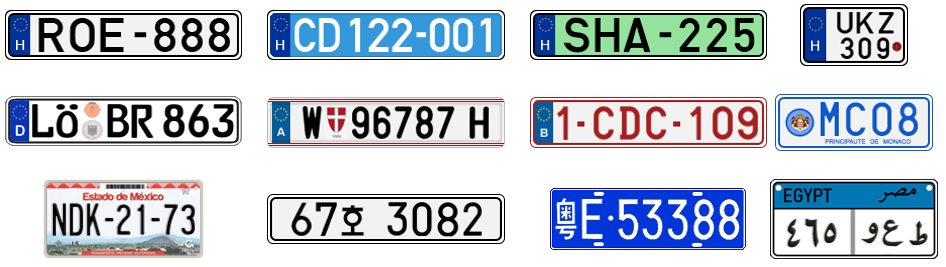
\includegraphics[width=.85\columnwidth]{.//Figure/OCR/plates.png}}
 \caption{License plates from Hungary (1st row), Europe (2nd row), and other continents (3rd row).}
 \label{fig:simple}
\end{figure}

A few characters are traditionally hard to distinguish in the Latin alphabet, like 0-O-Q or 1-I. This issue is often eliminated by prohibiting letters and numbers on the same character position. However, as plate structures can vary even in a single country, this is not a general solution. Moreover, two different characters may be the same in a font (like 0-O in the Mandatory) or across different fonts. Therefore, I decided that the unique items to distinguish are 0-9 and A-Z excluding O, plus the hyphen (10 + 25 + 1 characters). Other difficulties arise from picture quality and visibility aspects (lighting, contrast, rotation, motion-blur). This diversity suggests a general OCR solution has the edge in the long run over systems based on hand-crafted feature extraction for each plate type.

For this reason, I implemented a data generator, which approaches the task at the character level. It uses three types of resources to create an output: a list of characters to generate random text, fonts, and overlay images to mimic dirt, ice, and other phenomena. The generator handles text bounding boxes to be converted to output detector training data, and it can produce multiple text blocks. Creating one 50x500 grayscale image takes 10.934 ms. The generator applies data augmentation techniques to enrich data diversity.

\begin{algorithm}
  \caption{Data generator pipeline}
\begin{algorithmic}[1]
\label{alg:alg}
 \STATE \textbf{procedure} Generate($args$)
 \STATE random font and image overlay from $args$
 \STATE $bckgColor$ = random value [0...255] in every channel
 \STATE $image$: create with defined dimensions from $args$ and $bckgColor$
 \STATE $generatedTexts$ = $args[numBlocks]$ random texts in the range of 1...10.
 \STATE $lastBoxCoords$ = [0,0,0,0]
 \STATE $insertedTextIndices$ = []
 \FOR{$text$ in $generatedTexts$}
 \STATE $textColor$ = text and background colors must have at least 20\% diff in one channel (randomly selected which channel satisfy this)
 \STATE $textImage$: create text image from $text$, with a background color identical to $bckgColor$
 \IF{$textImage$ is bigger than $image$ in any dimension}
 \STATE $textImage$: resize to fit onto the $image$
 \ENDIF
 \STATE $textImage$: resize ratio with a value in the resize range (typically 0.85...1)
 \STATE $textImage$: random aspect ratio change, heigh, and width offset
 \IF{($lastBoxCoords[3]$ < $boxYstart$) || (($lastBoxCoords[2]$ < $boxXstart$) \&\& ($lastBoxCoords[1]$ < $boxYstart$))}
 \STATE $image$ += $textImage$
 \STATE $lastBoxCoords$ = [$boxXstart$, $boxYstart$, $boxXend$, $boxYend$]
 \STATE $insertedTextIndices$ += currentBoxIndex
 \ENDIF
 \ENDFOR
 \STATE $image$: random rotation and perspective transformation
 \STATE $image$: resize to the required size
 \STATE $image$ += random overlay with offset and rotation
 \STATE $image$: random brightness, contrast, sharpness, gaussian blur (within $args$ constraints)
 \STATE $image$: downscale between a range from $args$, then scale back
 \STATE $image$: normalize from [0...255] to [0...1), convert to float32
 \STATE $label$ += $text$ which Id is in $insertedTextIndices$
 \STATE $label$: encode $label$ to a number label with dictionary from $args$
 \STATE return $image$, $label$
 
\end{algorithmic}
\end{algorithm}

As the validation samples are also generated, the images must be equally distributed across different evaluation sets. A single epoch is set to contain 10,000 images. With this size, there is a maximum of +/-0.015 deviation in loss across multiple validations.

\begin{figure}[htb]
 \centerline{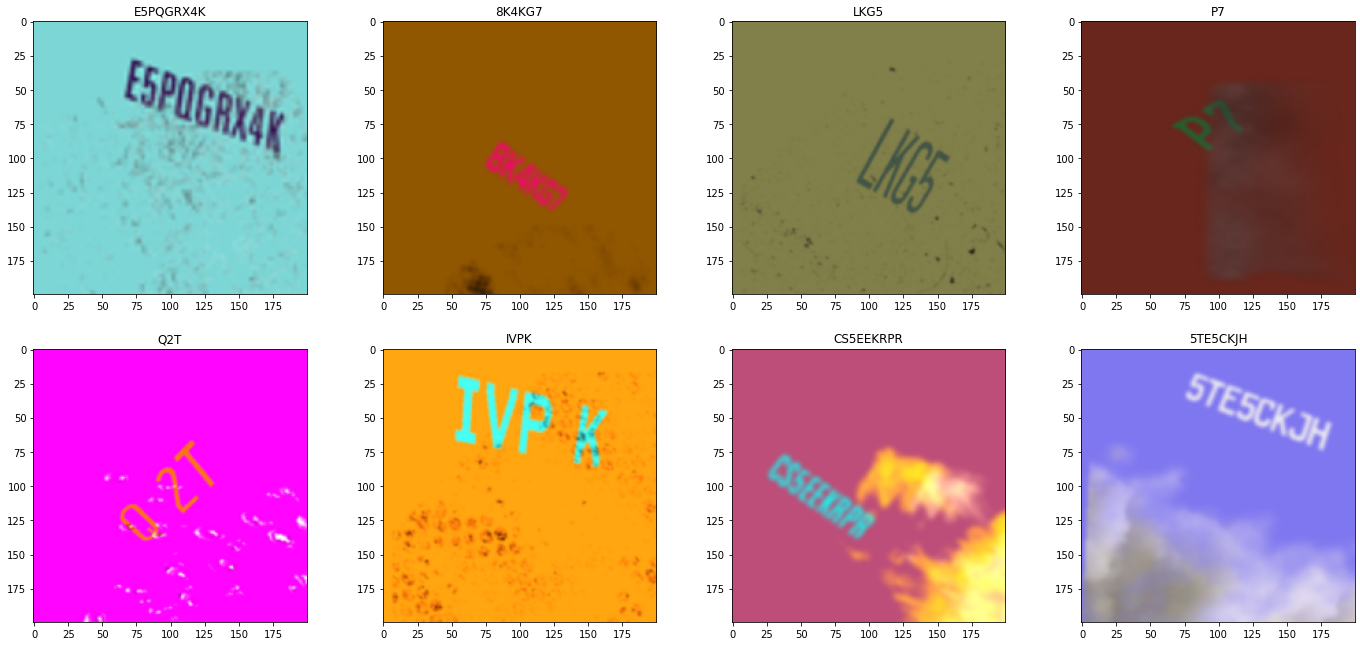
\includegraphics[width=.85\columnwidth]{.//Figure/OCR/generated.png}}
 \caption{One-line generated samples with labels on top. From the validation set, hard overlays have been removed so that the completely illegible characters do not affect results.}
 \label{fig:simple}
\end{figure}

\section{Model}

My OCR approach is based on feed-forward recurrent convolutional networks (CRNN) that produce fixed-size arrays of character probabilities.

\subsection{Connectionist Temporal Classification}

Connectionist Temporal Classification\cite{CTC} is used to compute model loss. The cost function has a barely documented Keras implementation, which I wrapped into a layer to make it easily detachable after training. This layer has two inputs: model prediction (\textit{batch\_size, max\_timesteps, num\_characters}) and ground truth encoded as numbers (\textit{batch\_size, max\_len}). Besides the 36 identifiable items, two more numbers are indicating the non-character token and the unknown character. Inputs must be the same length in a single batch. If a label's text is shorter than the maximum length, padding is expected with non-character tokens. The padding ensures that the model can be trained with greater batches than one, as multiple labels can be merged into a single, same dimensional array. The layer deduces the length of each label at runtime before computing its cost. To do that with arbitrary batches, I had to put a loop into the layer. The implemented TensorFlow loop is 30\% slower than the Python counterpart, but it can be placed on a TensorFlow graph.

\subsection{Building blocks}

A custom convolution layer is defined with Convolution $\rightarrow$ Nonlinearity $\rightarrow$ Dropout $\rightarrow$ Batch Normalization. These types of layers are stacked on top of each other in the residual blocks. The implementation allows to specify the type of activation function, the proportion of dropout, and whether to use Batch Normalization or not (when enabled, it adds bias to the output, so the convolution operation's bias is disabled in that case). Every convolution operation uses ``SAME'' padding. It applies padding so that the whole input gets fully covered by the filter and specified stride. The name comes from that, for stride 1, the size of the output is the same as the input. This partly solves the skewed kernels and feature-map artifacts issue induced by the operation\cite{PadBlindSpot}.

The main parts of the network are the residual blocks which consist of three components. The residual stage contains an arbitrary number of convolution layers with the same input/output size and channels. This block of layers is defined with a skip connection between the input and the output to overcome the vanishing gradient problem, which that means the block's input directly influences its output through a ``gradient highway'', not just through convolutions. After that, an upscaling convolution layer doubles the number of channels (it is the only layer that gradients cannot bypass; therefore, it is a bottleneck). It is followed by spatial downscaling by a factor of two with pooling. In this configuration, a block with input dimensions (height, width, channels) has an output of (\textit{height/2, width/2, channels*2}). My implementation was inspired by the ResNet\cite{ResNet} architecture.

\begin{figure}[htb]
 \centerline{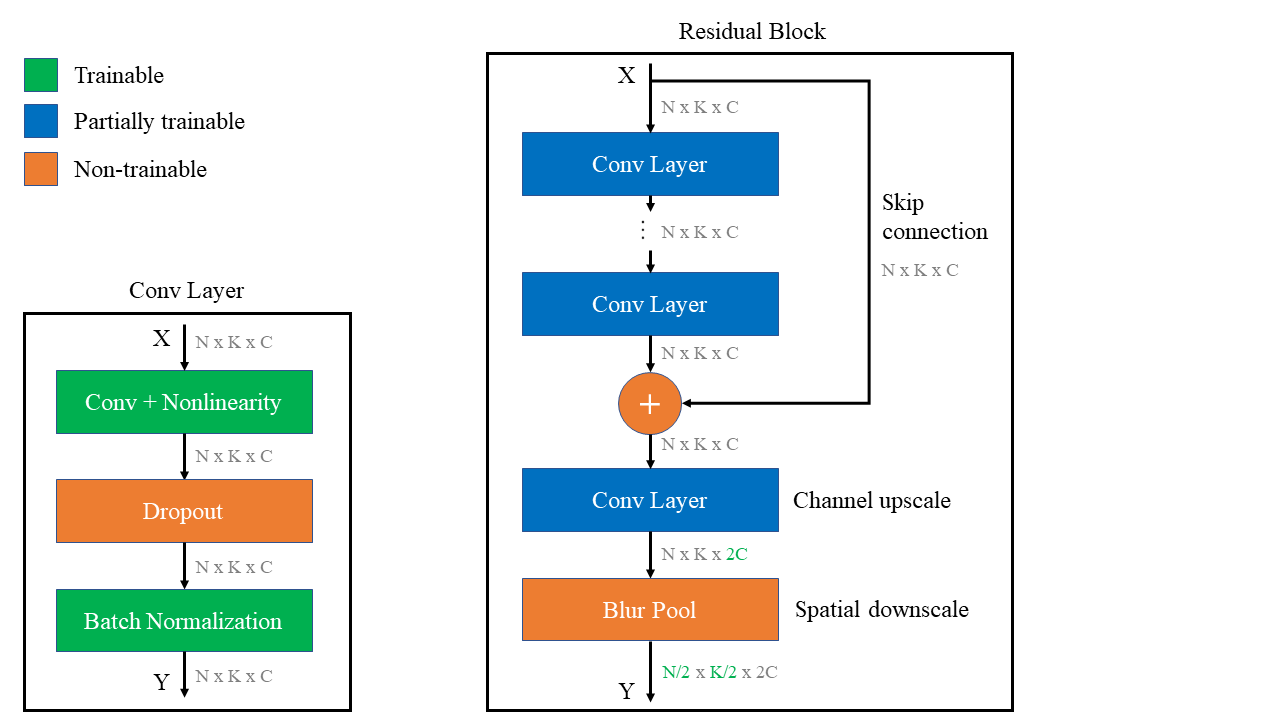
\includegraphics[width=.85\columnwidth]{.//Figure/OCR/Slide4.PNG}}
 \caption{Network building blocks with the convolution layer (a) and the residual block (b).}
 \label{fig:simple}
\end{figure}

In the recurrent part of the network, two Long Short-Term Memory\cite{LSTM} layers are stacked on top of each other responsible for sequential processing. In the network's first layer, the height and width dimensions of the input are swapped so that the width is the first dimension in the model. Thus, recurrent layers process inputs horizontally. A dense layer follows the last LSTM layer with a dimension of (\textit{input\_width * downscale\_factor, num\_characters}), which is the network's output matrix.

The best model has a downscale factor of three (number of residual blocks) and an input image width of 500 pixels, which means 63 steps overall. One window has a width of 8 pixels. Each window must be assigned to a real or an empty character token. It means that net 31 characters can be recognized to have enough space for characters and empty tokens in the output matrix.

\begin{figure}[htb]
 \centerline{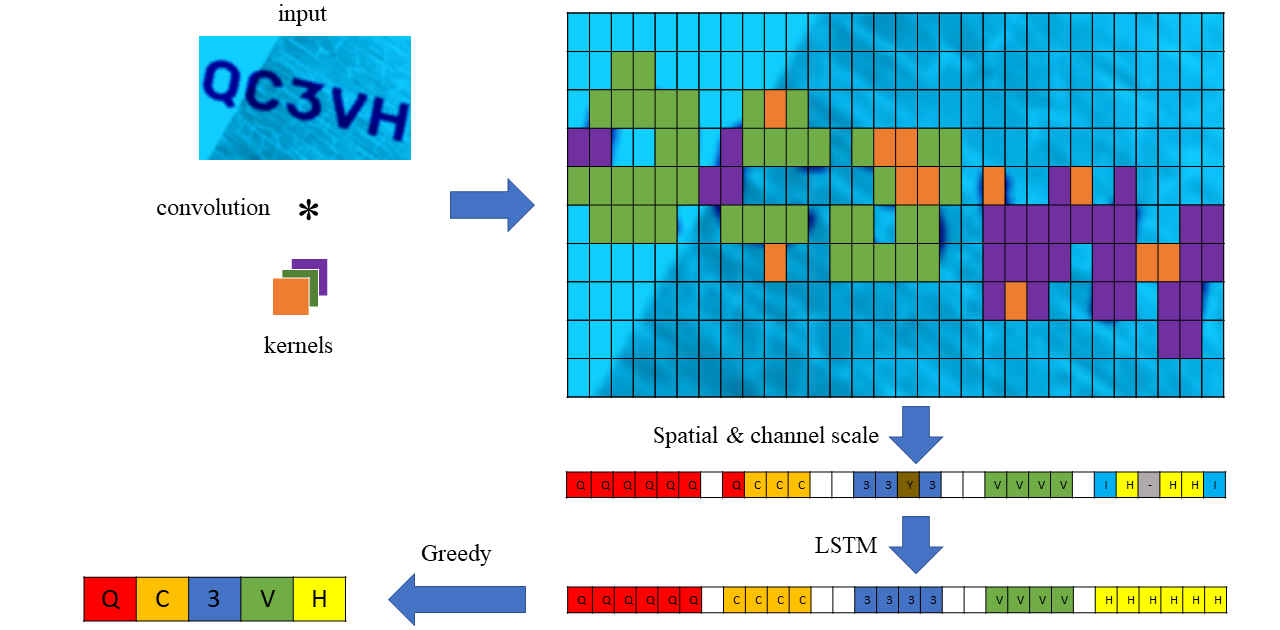
\includegraphics[width=.85\columnwidth]{.//Figure/OCR/Slide5.PNG}}
 \caption{Simplified representation of the network's key processing steps.}
 \label{fig:simple}
\end{figure}

\subsection{Greedy search}

In training, the CTC layer handles raw model outputs and ground truth labels, then calculates loss to backpropagate. However, this is not required for inference. Multiple approaches are available to decode raw outputs of the last dense layer. The Greedy solution keeps the maximum index at each step, then merges the same tokens between empty tokens. This way, multiple recognitions triggered by the same character are eliminated. The next step is to remove the empty tokens and decode the sequence with the model's vocabulary. That step produces the final text. Other approaches, like Beam search, iteratively create text candidates, arranges them based on their probability scores, and keeps the best ones after every iteration. The most probable beam at the end is returned as a result. This algorithm can be highly computation-intensive depending on the number of beams. Word Beam Search\cite{WordBeamSearch} takes this idea to another level: it constrains beams with a prefix tree of existing words. This solution can be helpful in situations where the words to recognize are from a specific vocabulary, but in the case of plate recognition, such a semantic assumption does not help. For these reasons, I implemented the Greedy algorithm.


\section{Experiments}

As a starting point, the model is trained with two residual blocks with a single convolution layer in each. The first block starts with 32 input channels, and the batch size is 8. Adam optimizer\cite{Adam} is used with the default parameters (1e-3 learning rate). One epoch is equal to 100,000 images, and early stopping is applied with five epoch patience. This model reached the optimum after 13 epochs with a validation loss of 0.2298.

\begin{table}[h]
\caption{The effect of batch sizes. Smaller batches converged faster at the beginning of training, but their improvement flattened out earlier at worse sub-optimal points. Batch size 128 was the largest that could fit into the memory.}
\noindent
\centering
\begin{tabular*}
{\columnwidth}{@{\extracolsep{\stretch{1}}}*{3}{r}@{}}
    & Epochs & Loss\\ \hline
    $batch 8$ & $8$ & $0.2121$ \\
    $batch 16$ & $29$ & $0.1545$ \\
    $batch 32$ & $22$ & $0.1134$ \\
    $batch 64$ & $55$ & $0.0855$ \\
    $batch 128$ & $51$ & $\textbf{0.0848}$ \\                   
\end{tabular*}
\end{table}

\subsection{Shift-invariance}

Zhang et al.\cite{Shift-Invariant} pointed out that modern CNNs lack shift-invariance since max-pooling, average-pooling, and strided-convolution ignore Nyquist's sampling theorem. The proposed solution is the use of blur-pooling, where spatial downsampling happens. I implemented blur-pooling with separable kernels and replaced all the other pooling layers with them. Although they claim that the solution is compatible with the layers listed above, I wanted to keep the number of layers as low as possible. The shift-invariant model slightly improved in loss, but a lot in the speed of convergence. Therefore, I continued to work with this model as the new benchmark.

\subsection{Hyperband optimization}

Hyperparameter optimization has been realized with the Hyperband algorithm\cite{Hyperband}. Another option considered was Bayesian optimization. I chose the former because adaptive Bayesian methods do not handle discrete, independent, unordered values well, and training would have lasted longer (since one configuration is done when the model training stops). Hyperband is a fast guided random search that works like a knockout sports competition: it generates combinations and trains them for a few epochs. After that, the top-performing part of the models is trained further, while the others are discarded. The iteration repeats until all the remaining models stop learning or there is a clear winner. 

Hyperband strongly filters models based on early training performances. Therefore, variable batch size or learning rate was not possible with this algorithm because smaller batches tend to outperform larger ones initially, but not in the long run. The selected parameters to optimize were the number of features of the first block (which is then doubled by every consequent block), kernel size, whether residual connections and batch norm layers are needed, dropout rate, number of blocks, convolutional layers in blocks, and type of activation function. A batch size of 32 was applied during training with every model, as instances with more blocks and layers should also fit into memory. Therefore, the previous Batch 32 model served as a baseline.

\begin{table}[htb]
\caption{Top3 configurations found by Hyperband. Only the top2 were trained until convergence, the 3rd has been stopped earlier. Columns: model, features, kernel, residual, batch norm, dropout, blocks, layer per block, activation, epochs, loss.}
\noindent
\centering
\begin{tabular*}
{\columnwidth}{@{\extracolsep{\stretch{1}}}*{11}{r}@{}}
    & Feat & Ker & Res & BN & Drop & B & L & Act & Epochs & Loss\\ \hline
    $base$ & $32$ & $3$ & $\checkmark$ & $\checkmark$ & $0.1$ & $2$ & $1$ & $ReLU$ & $22$ & $0.1134$ \\
    $1st$ & $64$ & $3$ & $\checkmark$ & $\checkmark$ & $0.09$ & $3$ & $3$ & $ReLU$ & $39$ & $\textbf{0.0753}$ \\
    $2nd$ & $64$ & $5$ & $X$ & $\checkmark$ & $0.2$ & $2$ & $2$ & $ReLU$ & $35$ & $0.0862$ \\
    $3rd$ & $64$ & $3$ & $X$ & $\checkmark$ & $0.3$ & $2$ & $3$ & $ELU$ & $15$ & $0.1554$ \\                            
\end{tabular*}
\end{table}

\begin{figure}[htb]
 \centerline{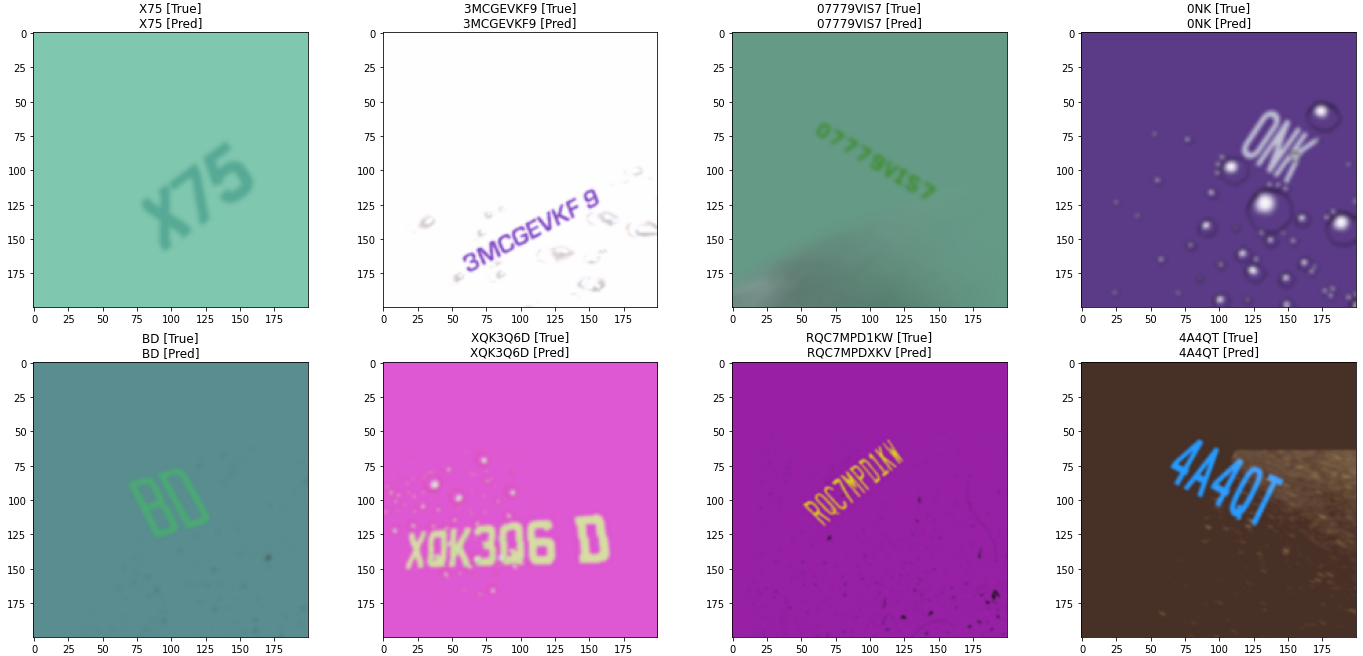
\includegraphics[width=.85\columnwidth]{.//Figure/OCR/inference.png}}
 \caption{Inference results of the best performing network.}
 \label{fig:simple}
\end{figure}

\section{Multiline recognition}

There are numerous approaches to process number plates with multiple lines. One can be the usage of object detection to detect individual text blocks on an image. One powerful model based on this approach is the CRAFT\cite{CRAFT} text detector. Another approach is text segmentation, which is not necessarily done by neural networks. In both cases, however, the recognition of text blocks and characters are separated steps and the weights used for them are not shared. I experimented with a model that merges these steps. The key idea is to add some layers to the end of the network that learns to unfold the 2-dimensional feature map into a tall, 1-dimensional feature sequence. This approach changes the main axis (the horizontal reading of text changes to process vertical features). To accomplish this, I implemented a modified Origami\cite{OrigamiNet} module that includes convolution layers and resizing with bilinear interpolation.

 \begin{algorithm}
     \caption{Pseudo code of the Unfolding module}
 \begin{algorithmic}[1]
  \label{alg:alg}
    \STATE \textbf{procedure} Unfolding($inDim, inChannel, outChannel, numBlocks, numLayers$)
    \STATE vertical = inputDim[0]
    \STATE horizontal = inputDim[1]
    \FOR{$i = 0$; $i$ $<=$ $numBlocks$; $i$++}
    \STATE vertical *= 2
    \STATE horizontal /= 2
    \STATE Resizing(vertical, horizontal, interpolation=bilinear)
    \FOR{$j = 0$; $j$ $<=$ $numLayers$; $j$++}
    \STATE Conv(inChannel, inChannel)
    \ENDFOR
    \ENDFOR
    \STATE Conv(inChannel, outChannel, (1, 1), (1, 1))
    \STATE xDownFactor = pow(2, $numBlocks$)
    \STATE xRemain = inDim[1] \% xDownFactor > 0
    \STATE xLastKernelSize = (inDim[0] // xDownFactor) + xRemain
    \STATE Conv(outChannel, outChannel, (1, xLastKernelSize), (1, xLastKernelSize))
\end{algorithmic}
\end{algorithm}

The original solution was not ideal for this task. I had to remove the recurrent part of the original network (LSTM layers) because they introduced instability while training. I replaced pooling with strided convolution, increased the number of resizing steps, reduced the spatial rescaling ratio, and increased the number of convolution layers. After these modifications, the module started working as intended. The best loss was 0.9517 on images with a maximum of five rows of texts after 73 epochs (0.0991 on single line images). It is far from an optimal solution, but all I had to do is to add a module to the end of an existing model. Unfolding also scales well, as the runtime does not change even when processing multi-row text images.

However, unfolding has its drawbacks. The original model had a size of 640 KB, while this module increased it to 3.138 MB. Multiplying the size of a model already reading single-line texts five times seems wasteful (even so, it is less than using a separate detector and a single line recognizer). Another problem is that unfolding struggles with rotated texts. It jumps through the lines while reading when rotation is close to 45 degrees. Therefore, in my opinion, this solution is not adequate for this task unless I apply an extra horizontal transformation step.
